\section{Project Management}
\label{sec:project_management}
\lhead{\thesection \space Project Management}

Project management is used for the success of projects, a project is a unique single endeavour. To proper manage a project to success, certain skills are needed. Communication, proper documenting and risk management are just some of them. In the world of software development, scrum is a well-established way of managing projects. This chapter includes the most relevant topics in terms of project management based on the \textit{Connected.Football} application.


%%%%%%%%%%%%%%%%%%%%%%%%%%%%%%%%%%%%%%%%%%%%%%%%%%
%% INTEGRATION MANAGEMENT
%%%%%%%%%%%%%%%%%%%%%%%%%%%%%%%%%%%%%%%%%%%%%%%%%%

\subsection{Integration Management}
\label{ssec:integration_management}

Project Integration Management includes the processes and activities to identify, define, combine, unify, and
coordinate the various processes and project management activities within the Project Management Process
Groups.
\newpage

\subsubsection{Develop Project Charter}
\label{sssec:develop_project_charter}

The created project charter below helps to identify the key information in the project.
All necessary data about the customer and project related risks or issues related to the budget are tackled.

\begin{figure}[H]
  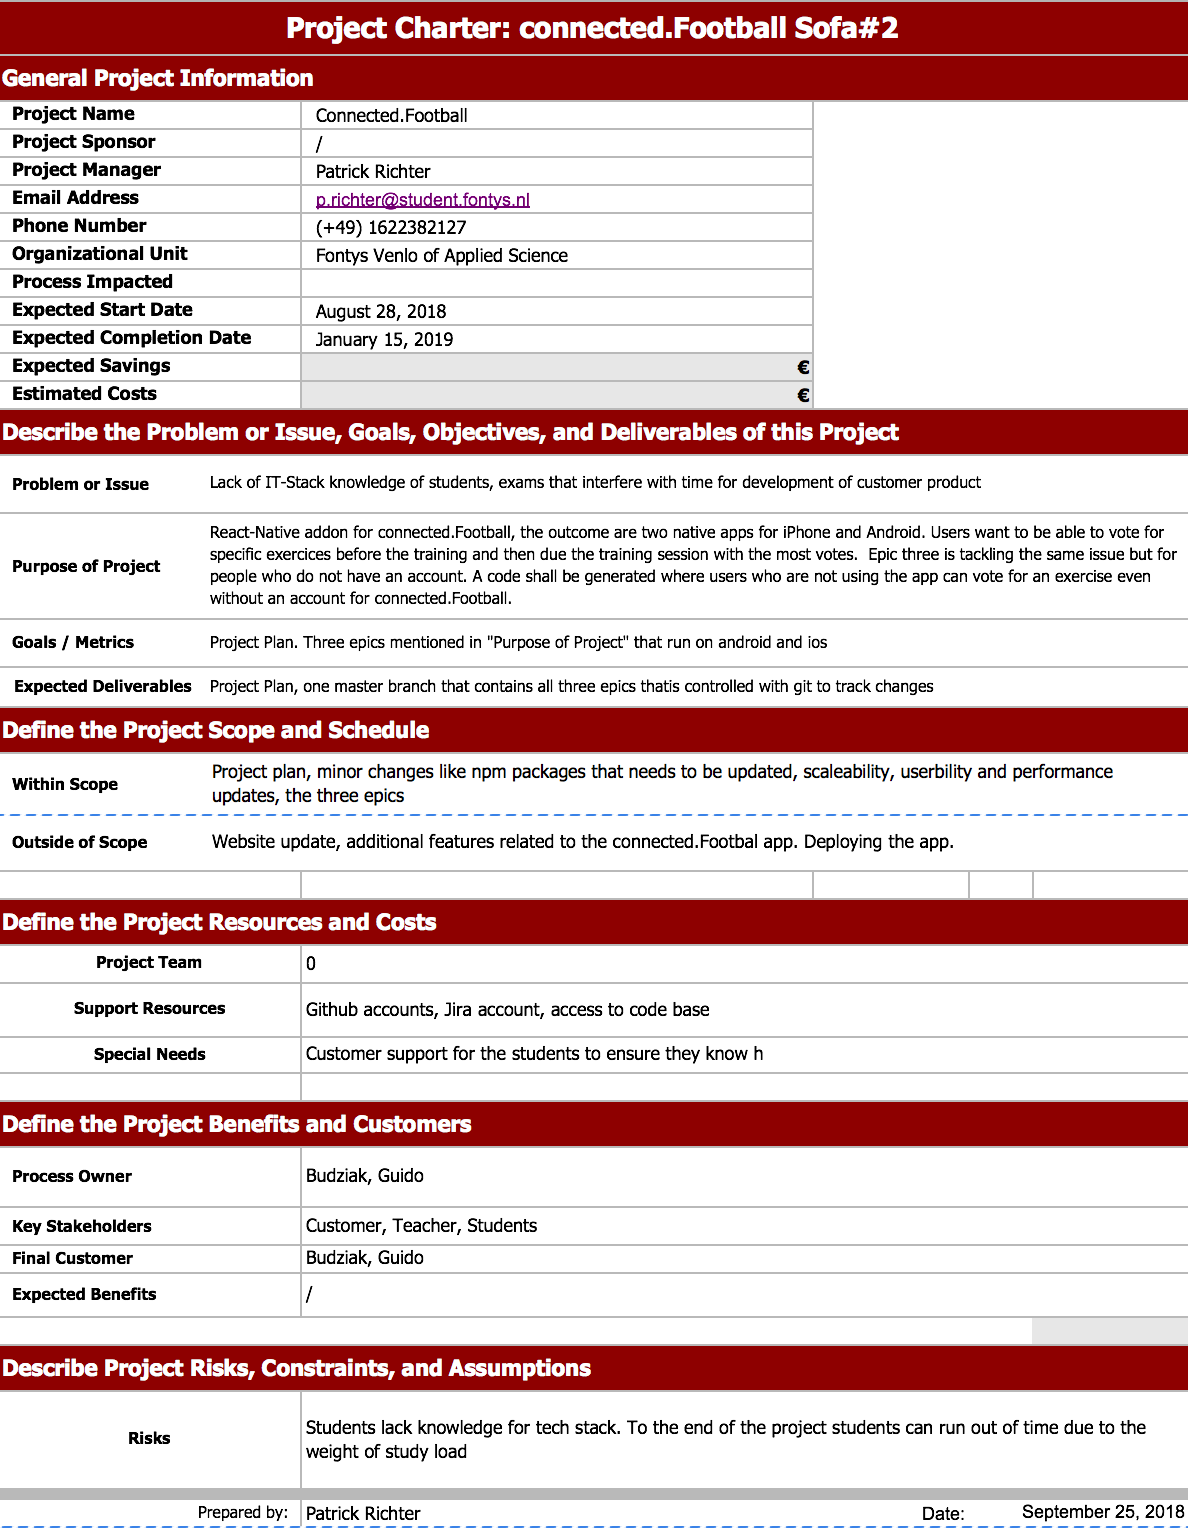
\includegraphics[width=425px, height=585px]{images/projectChater.png}
  \caption{Project Charter}
  \label{fig:project_charter}
\end{figure}

\subsubsection{Perform Integrated Change Control}
\label{sssec:perform_integrated_change_control}

A detailed change proposal describes why the change is needed, expected outcomes and impacts, time and resources required, and any other factors that need to be reviewed. 
In this project there is no change control board (CCB), the project is too small to implement it, so the group decided to skip it. All necessary information and updates are shared directly in the group. Customer related information were shared in the customer meeting.

\subsubsection{Close Project or Phase}
\label{sssec:close_project}

At the end of the project, the created \textit{GitHub}, \textit{Jira} and Apple Developer accounts for the students will be returned to the project owner. \newline
After project completion, students will pursue their major and head on to their bachelor thesis.\newline
Besides that, there is no more equipment that has to be returned.


%%%%%%%%%%%%%%%%%%%%%%%%%%%%%%%%%%%%%%%%%%%%%%%%%%
%% SCOPE MANAGEMENT
%%%%%%%%%%%%%%%%%%%%%%%%%%%%%%%%%%%%%%%%%%%%%%%%%%

\subsection{Scope Management}
\label{ssec:scope_management}

Scope management is what is done to make sure that the project includes all the work relevant to achieving the project’s objectives and not anything else. It’s about controlling what is included in the project and what is not.

\subsubsection{Plan Scope Management}
\label{sssec:plan_scope_management}

This project involves designing, programming, and testing a new software product which will be a new module of the \textit{Connected.Football} application to add a feature to vote on given exercises. This includes design of the software, all programming and coding, and testing/validation of the software.
\newline
For this project, scope management was the sole responsibility of all group members. The scope for this project is defined by the Scope Statement, Work Breakdown Structure and the Software Requirement Specification. Proposed scope changes may be initiated by the product owner as well as every member of the team.

\begin{table}[H]
    \centering
    \begin{tabular}{|c|c|l|}
        \hline
        \cellcolor{gray}Name & 
        \cellcolor{gray}Role &
        \cellcolor{gray}Responsibilities \\\hline
        Guido Budziak & Product owner &- Approve or deny scope changes.\\&&- Evaluate need for scope change requests.\\&&- Accept project deliverables\\\hline
        Lucas Gehlen&Team member&- Measure and verify project scope.\\
        Marco Kull&&- Update project documents upon scope changes.\\
        Patrick Richter&&- Measure and verify project scope.\\
        Sebastian Wilczek&&- Participate in defining change resolutions.\\
        &&- Evaluate the need for scope changes.\\\hline
    \end{tabular}
    \caption{Scope Roles \& Responsibilities}
    \label{tab:scope_roles}
\end{table}

\subsubsection{Collect Requirements}
\label{sssec:collect_requirements}

The requirements for this project are delivered by the product owner. During the weekly meetings with the product owner the team discussed the design fragments with them to ensure the requirements are met. All requirements were documented in a software requirement specification document.

\subsubsection{Define Scope}
\label{sssec:define_scope}

This project includes the design, programming, and testing of a new module of the \textit{Connected.Football} application to add a feature to vote on given exercises. The deliverables for this project is a completed module with the flexibility to modify and expand as necessary in the future. This project will be accepted once the new module has been successfully tested. Assumptions for this project were that support was to be provided by the project owner.

\subsubsection{Create WBS}
\label{sssec:create_wbs}

The project is broken down into three phases: Vote4Fun; Promotion Code; and Vote4Fun Group Extension. Each of these phases is then subdivided further down.

\begin{figure}[H]
	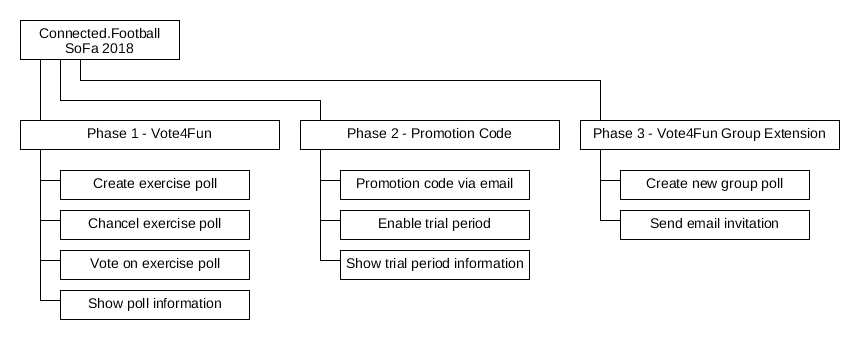
\includegraphics[width=\textwidth]{images/wbs.png}
	\caption{Work Breakdown Structure}
    \label{fig:wbs}
\end{figure}

\subsubsection{Validate Scope}
\label{sssec:validate_scope}
    
As this project progressed the team verified interim project deliverables against the original scope. To ensure that project work remains within the scope of the project those interim deliverables were discussed in weekly meetings with the product owner.

\subsubsection{Control Scope}
\label{sssec:control_scope}

The project team worked together to control the scope of the project. The project manager oversaw the project team and the progression of the project to ensure that this scope control process if followed.
\newline
If a change to the project scope is needed, all team members and the product owner must approve of the scope change.


%%%%%%%%%%%%%%%%%%%%%%%%%%%%%%%%%%%%%%%%%%%%%%%%%%
%% TIME MANAGEMENT
%%%%%%%%%%%%%%%%%%%%%%%%%%%%%%%%%%%%%%%%%%%%%%%%%%

\subsection{Time Management}
\label{ssec:time_management}

Project Time Management includes the processes required to manage the timely completion of the project. Proper time management helps understand what can realistically be achieved in time. Ensuring that every milestone and working package has enough time assigned with a buffer if something goes wrong so the project stays in time.

\subsubsection{Plan schedule}
\label{sssec:plan_schedule}

In the \textit{Connected.Football} project requirements got defined, working tasks and responsible person with a scheduled time are assigned to each task. Figure \ref{fig:overview_tasks} shows how it was planned.

\begin{figure}[H]
  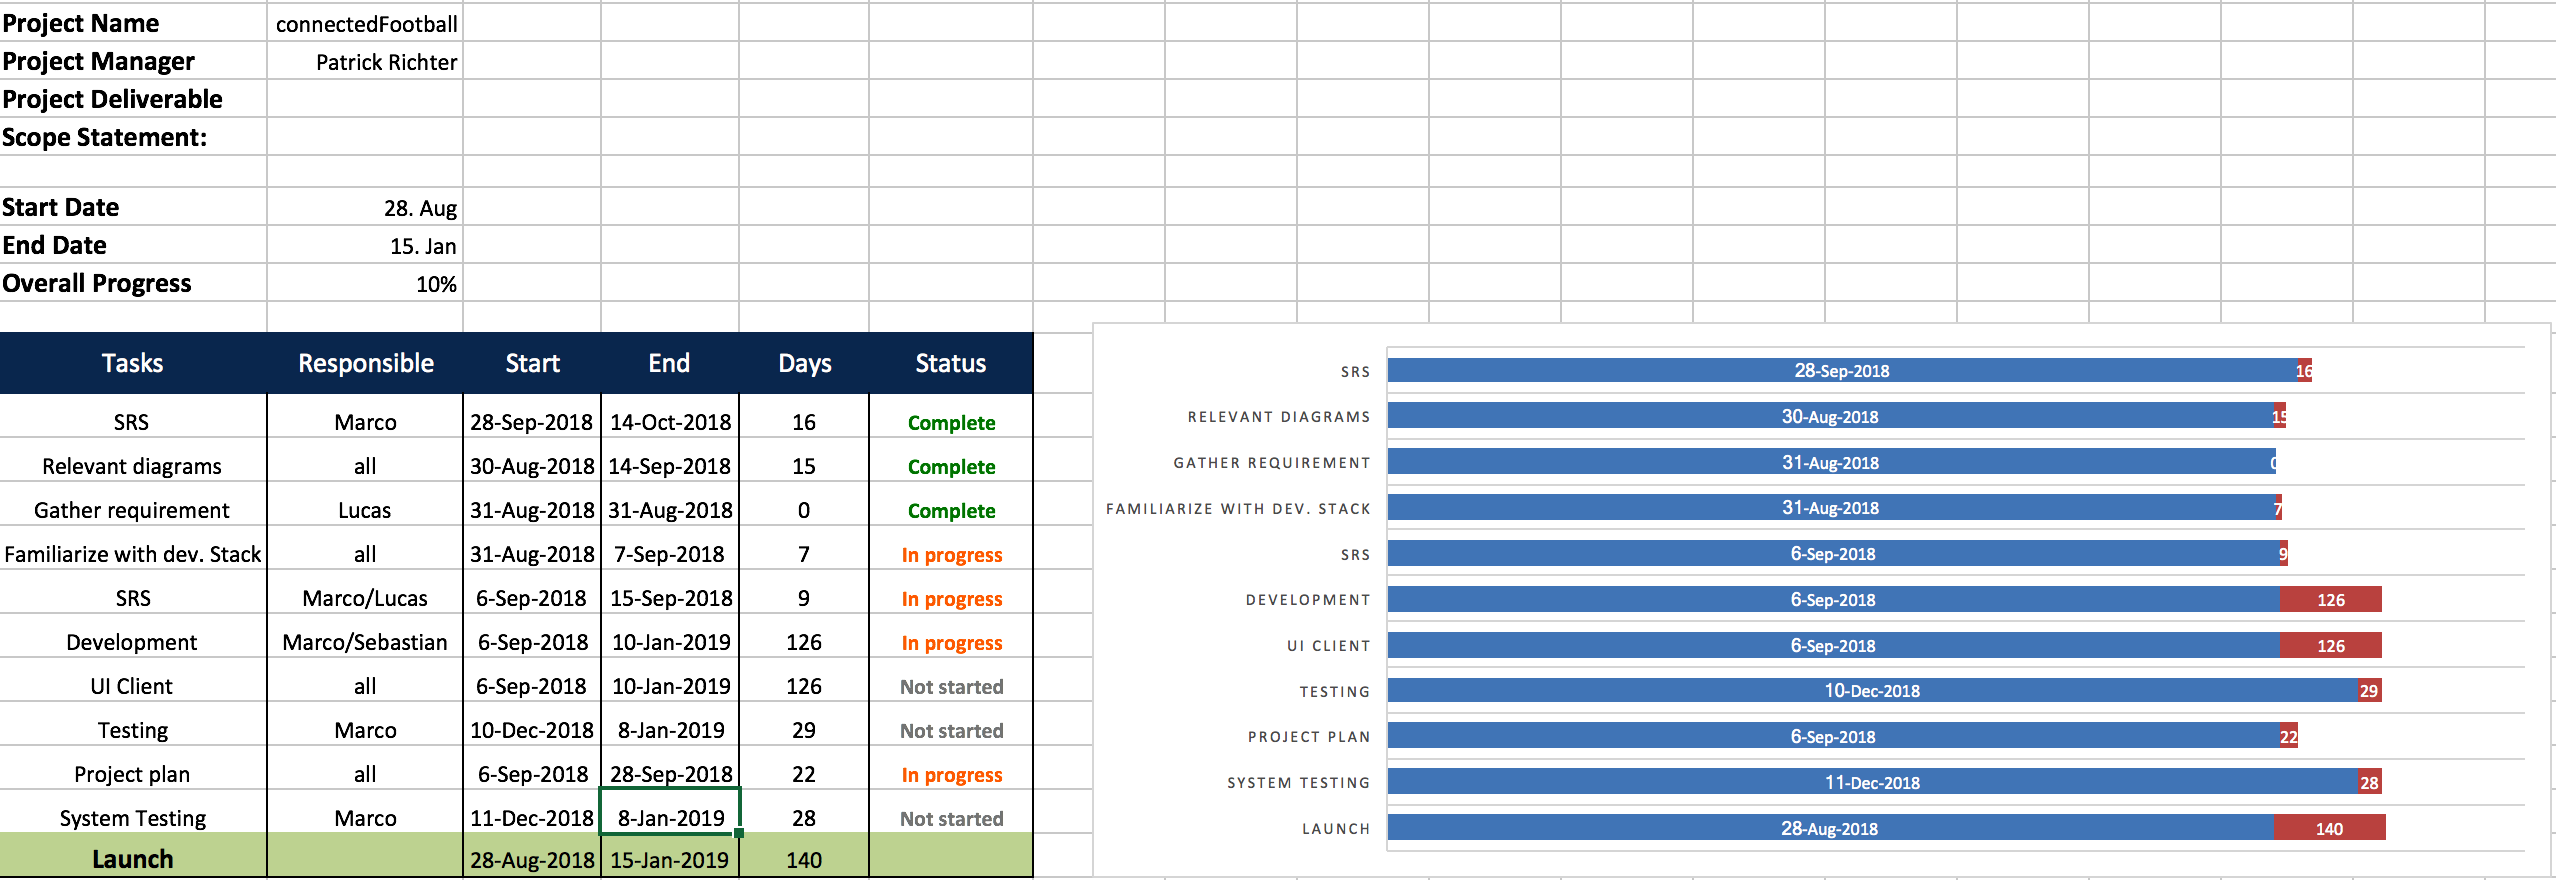
\includegraphics[width=\linewidth]{images/diagrams/timemangement.png}
  \caption{Overview Tasks}
  \label{fig:overview_tasks}
\end{figure}

On the right side we see a blue line with the activities. The numbers at the end of the scale with a red background are the indicated days that are needed to achieve the task. This schedule has been created at the beginning of the project and is updated continuously. 

\subsubsection{Define Activities}
\label{ssec:define_activities}

To get an even more detailed overview of the project tasks the activities got defined on a lower level. A \textit{Work Breakdown Structure} (WBS) was created therefore. This WBS helps to get a better overview of the single tasks. In this case everybody got assigned to every task which actually makes no sense but in the beginning of the project everybody has to work on every task, even the scrum master has to develop. Therefore, it was decided to assign everybody to every task. The development tasks got broken down in even lower level steps so the developers know exactly on what they have to work on during a sprint. Only WBS point 4 was filled completely. Over the project life cycle this information was updated.

\begin{figure}[H]
  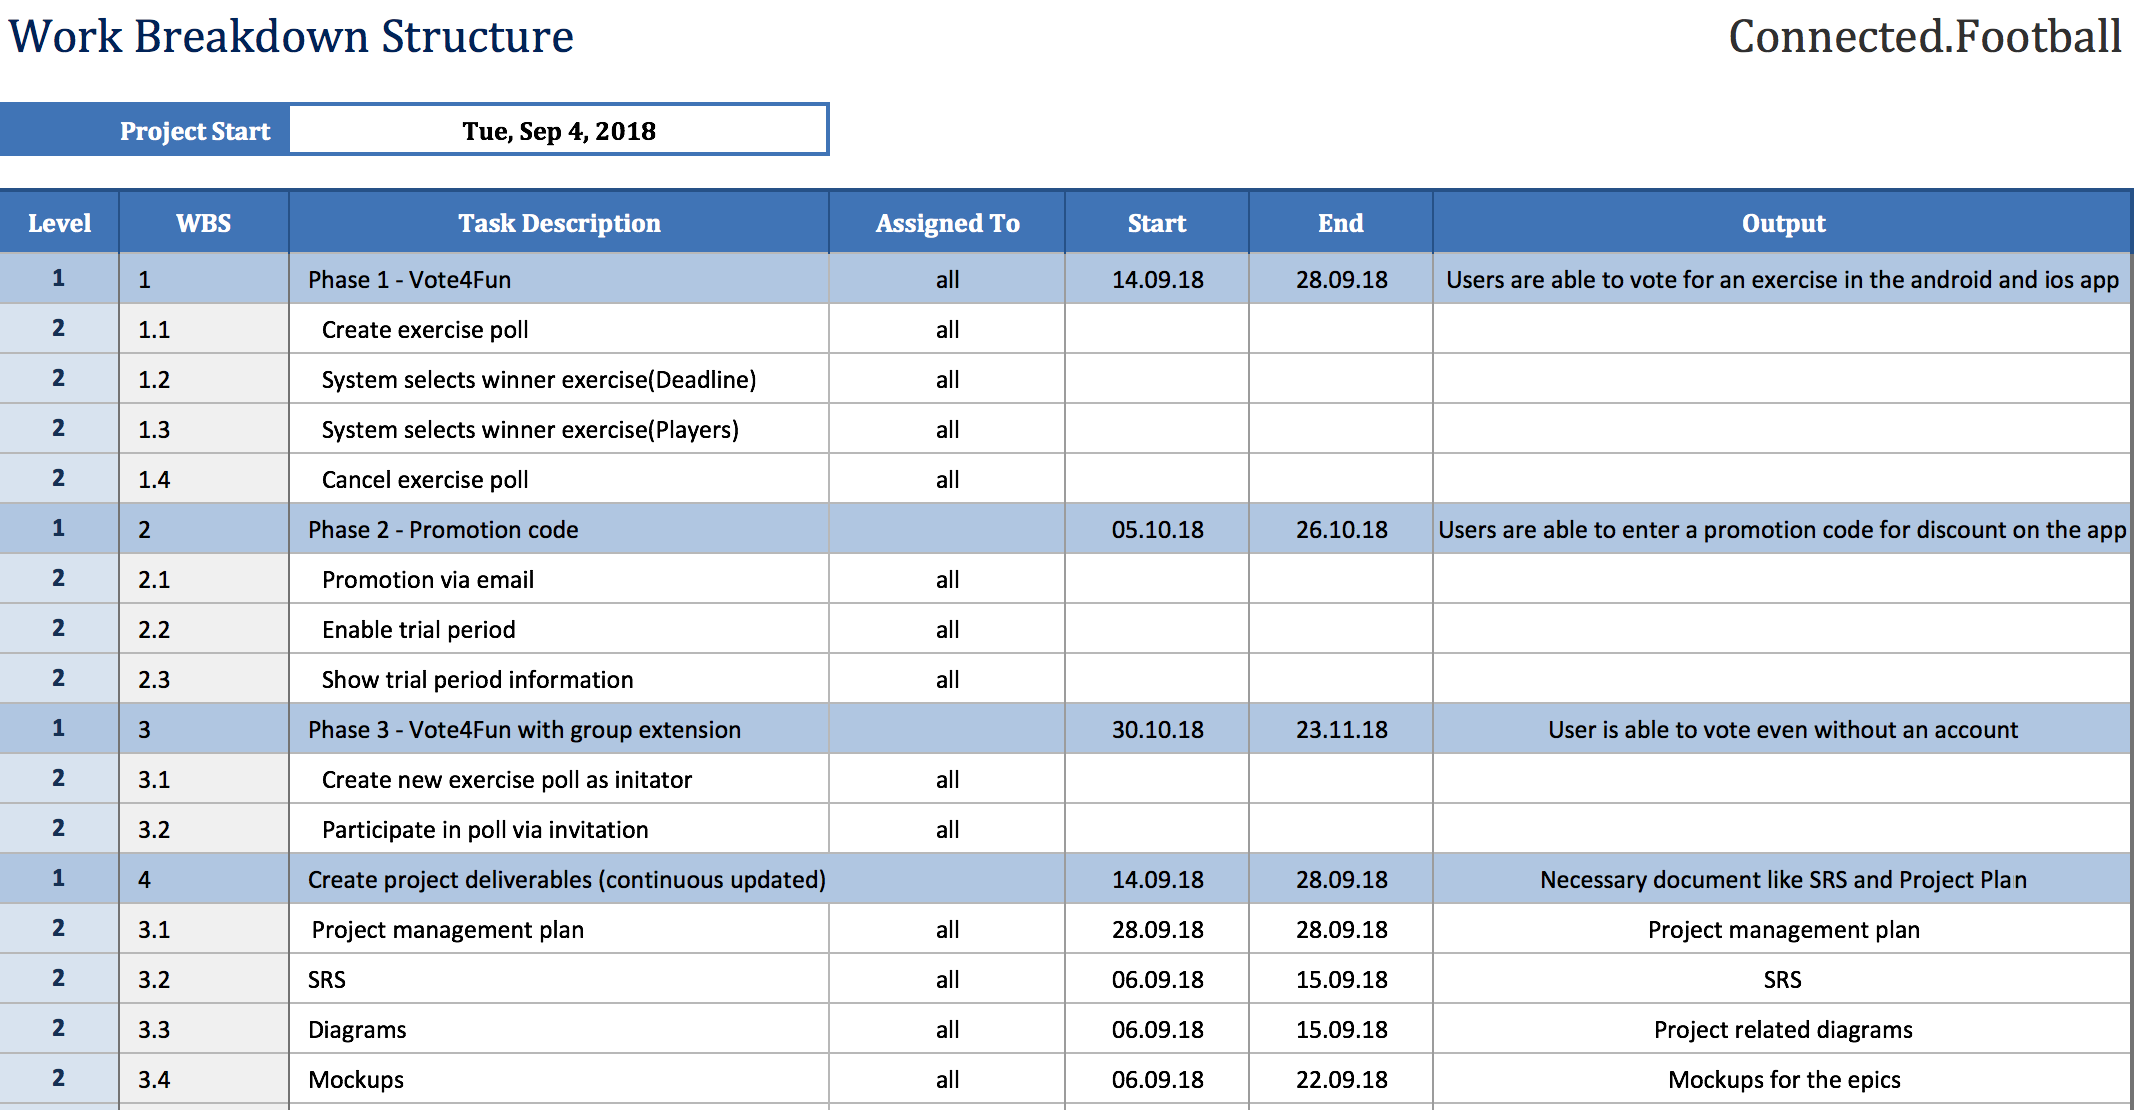
\includegraphics[width=\linewidth]{images/diagrams/wbs_detailed.png}
  \caption{WBS detailed overview of development}
\end{figure}

What is not mentioned here are smaller sub tasks e.g. updating \textit{React Native} or fixing bugs to make the application run on both devices. In particular one team member had issues making the program run on \textit{iOS} which took him in total 12 hours of work ending up deploying the software on an \textit{Android} device too because an activity like this consumes too much time and other more important task would suffer on completion.

\subsubsection{Estimate Activity Resources Process}
\label{sssec:estimate_activity_resources_process}

To achieve these activities certain resources are needed. In the project four people worked towards the success of the project. A detailed overview of the human resources and their related tasks can be found in chapter \textit{\ref{ssec:human_resource_management} \nameref{ssec:human_resource_management}}. For a proper working environment the project members got supplied with \textit{Jira} and \textit{GitHub} accounts, further details are found in \textit{\ref{ssec:procurement_management} \nameref{ssec:procurement_management}}.


%%%%%%%%%%%%%%%%%%%%%%%%%%%%%%%%%%%%%%%%%%%%%%%%%%
%% COST MANAGEMENT
%%%%%%%%%%%%%%%%%%%%%%%%%%%%%%%%%%%%%%%%%%%%%%%%%%

\subsection{Cost Management}
\label{ssec:cost_management}

This subsection deals with the cost management of the project in question. It is being detailed how cost were managed in the project and how costs and expenses were monitored over the course of the project.
\newline
Costs did not play a vital role in the project. Given that the project is part of a University module, the project team is working without compensation and all resources, such as they are mentioned in \textit{Subsection \ref{ssec:procurement_management}}, are being provided by the client.
\newline
Cost management was considered during the project planning due to the small likelihood that the project requires further resources. In this case, the responsibility for providing these resources were that of the client. However, the project team would have been responsible for defining why the new resource is necessary for development and on what scale the resource needs to be provided. However, such a case never occurred during the course of the project is only mentioned for the purpose of completeness.


%%%%%%%%%%%%%%%%%%%%%%%%%%%%%%%%%%%%%%%%%%%%%%%%%%
%% STAKEHOLDER MANAGEMENT
%%%%%%%%%%%%%%%%%%%%%%%%%%%%%%%%%%%%%%%%%%%%%%%%%%

\subsection{Stakeholder Management}
\label{ssec:stakeholder_management}

Stakeholder Management includes the processes required to identify the people, groups and organisations that could affect or be affected by the project, to analyse stakeholder expectations and their impact on the project, and to develop appropriate strategies and tactics for effectively engaging stakeholders in a manner appropriate to the stakeholders interest and involvement in the project. Stakeholder Management helps to ensure that stakeholders are effectively involved in project decisions and execution throughout the life cycle of the project, to gain support for the project and anticipate resistance, conflict, or competing objectives among the project’s stakeholders.

\subsubsection{Identify Stakeholders}
\label{sssec:identify_stakeholders}

In order to develop an effective plan for managing stakeholders, they first need to be clearly identified and assessed. Stakeholders were identified by performing a stakeholder analysis in which potential stakeholders and relevant information (interests, involvement, inter dependencies, influence, and potential impact on project success) are gathered, documented and analysed. 


\begin{table}[H]
    \centering
    \begin{tabular}{|c|c|}
        \hline
        \cellcolor{gray}Name & \cellcolor{gray}Description \\ \hline
        Guido Bruzniak & Product owner \\ \hline
        Marco Kull & Quality Manager \\ \hline
        Sebastian Wilczek & Software Architect \\ \hline
        Patrick Richter & Project Leader \\ \hline
        Lucas Gehlen & Scrum Master \\ \hline
        Thijs Dorssers & Docent \\ \hline
    \end{tabular}
    \caption{Stakeholders}
    \label{tab:stakeholders}
\end{table}

For this project six stakeholders were identified. To assist with stakeholder identification and analysis, the team has created and is completing a Stakeholder Analysis Register categorised by Stakeholder Group. The Stakeholder Analysis Register captures the following information.

\begin{itemize}
    \item Group Name
    \item Number of Stakeholders in the Group
    \item Description of the Group
    \item Level of Impact on the Project
    \item Level the Group is Impacted by Project
    \item Current Change Readiness State
    \item Desired Change Readiness State
\end{itemize}

A snapshot from the Stakeholder Analysis Register is provided below.
Please note: Impact is measured by High (H), Medium (M) or Low (L).  State of change readiness is assessed using the measures from \textit{Project Management Body of Knowledge} (PMBOK) 5th Edition  as follows: 

\begin{itemize}
    \item U - Unaware – this group has no information about the project
    \item R – Resistant – aware of project and resistant to the changes and impacts the project may bring
    \item N – Neutral – aware of the project and neither supportive nor resistant
    \item S – Supportive – aware of the project and the potential changes and impacts and is supportive 
    \item L – Leading – aware of the project and actively engaged to ensure the project’s success
\end{itemize}

\begin{table}[H]
    \centering
    \begin{tabular}{|c|c|c|c|c|c|c|}
        \hline
        \cellcolor{gray}\begin{tabular}{@{}c@{}}Group\\Name\end{tabular} & \cellcolor{gray}\# in Group & \cellcolor{gray}Description & \cellcolor{gray}\begin{tabular}{@{}c@{}}Impact on\\Project\end{tabular} & \cellcolor{gray}\begin{tabular}{@{}c@{}}Impacted by\\Project\end{tabular} & 
        \cellcolor{gray}\begin{tabular}{@{}c@{}}Current\\State\end{tabular} & \cellcolor{gray}\begin{tabular}{@{}c@{}}Desired\\State\end{tabular}  \\ \hline
        \begin{tabular}{@{}c@{}}Project\\Team\end{tabular} & 4 & \begin{tabular}{@{}c@{}}The project\\team\end{tabular} & High & Low & L & L \\ \hline
        \begin{tabular}{@{}c@{}}Product\\Owner\end{tabular} & 1 & \begin{tabular}{@{}c@{}}The product\\owner\end{tabular} & High & High & L & L \\ \hline Coach & 1 &
        \begin{tabular}{@{}c@{}}The coach\\of the \\ project team\end{tabular} & Low & Low & S & S \\ \hline
    \end{tabular}
    \caption{Stakeholder Analysis Register}
    \label{tab:stakeholder_analysis_register}
\end{table}

As mentioned above, the \textit{Connected.Football} SoFa project is assessing each group’s position, as well as their impact on the project and/or how they are impacted by the project.  One purpose of this activity is to help identify and categorise groups so that appropriate attention can be given to each group according to the level of engagement needed. To help in this process, the project team made use of the PMBOK Power/Interest Grid to categorise each stakeholder group.  The Power/Interest Grid analyses stakeholder groups in a visual manner to further establish stakeholders level of interest or concern and their ability to influence the project outcomes. 
\newline
An important outcome of the stakeholder identification and analysis work, including the Power/Interest Grid, is to identify the most influential and most impacted stakeholder groups so that a focused stakeholder management strategy and plan can be developed and executed.

\begin{figure}[H]
  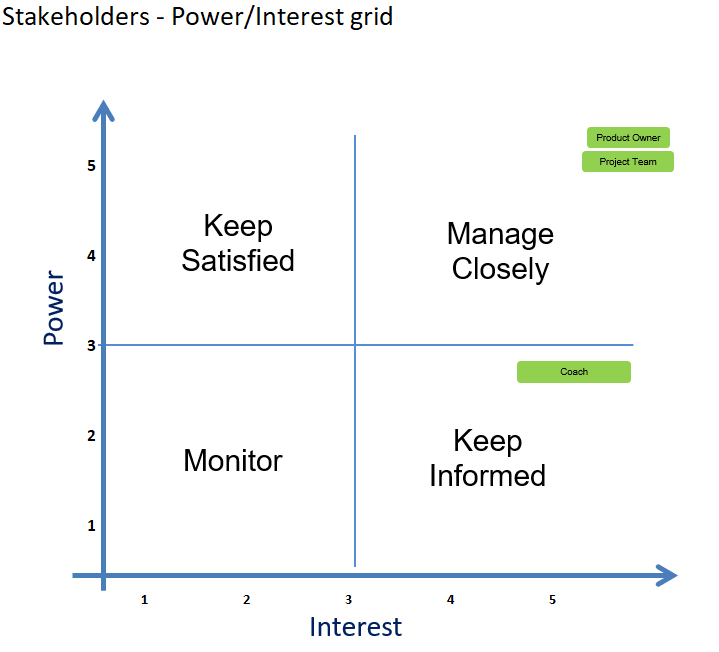
\includegraphics[width=\linewidth]{content/diagram/stakeholder/power_interest.png}
  \caption{Power/Interest Matrix}
\end{figure}

In addition, optional qualitative interviews may be performed for the Stakeholder Groups identified as most influential or most impacted by the project to validate that their issues and concerns have been captured accurately.

\subsubsection{Plan Stakeholder Management}
\label{sssec:plan_stakeholder_management}

Based upon the information gathered in the Stakeholder Analysis Register and the Communication Management, the Project Manager was responsible for engaging stakeholders throughout the life cycle of the project. The level of engagement required for each stakeholder may vary over the course of the project. For example, during the beginning stages of the project, it might be necessary for the Project Manager to engage key stakeholders to be highly engaged.  Highly engaged key stakeholders in the early stages of the project are pivotal for project kickoff, achieving staff buy-in and clearing obstacles. As the project progresses, the level of engagement shifted from key stakeholders to the broader project team and end-users.  
\newline
To ensure the correct level of engagement is being achieved by each stakeholder, the Project Manager analysed current levels of engagement by using the PMBOK Stakeholders Engagement Assessment Matrix.  As noted above in the Stakeholder Analysis Register, each stakeholder group was assessed in terms of their current and desired level of engagement.
 
 \begin{table}[H]
    \centering
    \begin{tabular}{|c|c|c|c|c|c|}
        \hline
        \cellcolor{gray}Stakeholder & \cellcolor{gray}Unaware & 
        \cellcolor{gray}Resistant & \cellcolor{gray}Neutral & 
        \cellcolor{gray}Supportive & \cellcolor{gray}Leading\\ \hline
        Guido Budziak & / & / & / & / & C/D \\ \hline
        Marco Kull & / & / & / & / & C/D   \\ \hline
        Sebastian Wilczek & / & / & / & / & C/D   \\ \hline
        Patrick Richter & / & / & / & / & C/D    \\ \hline
        Lucas Gehlen & / & / & / & / & C/D   \\ \hline
        Thijs Dorssers & / & / & / & C/D  & / \\ \hline
    \end{tabular}
    \caption{Stakeholder Engagement Assessment Matrix}
    \label{tab:stakeholder_engagement_assessment_matrix}
\end{table}

\subsubsection{Manage Stakeholder Engagement}
\label{sssec:manage_stakeholder_engagement}

To effectively manage stakeholder engagement, the \textit{Connected.Football} SoFa project utilised the Communication Management part and strategies identified above to communicate project related information to key stakeholders in a proactive and timely manner.  Leveraging the information provided in the Communication Management (i.e., stakeholder groups, communication items, purpose, method of communication, and frequency), the project had the ability to increase support and minimise stakeholder resistance throughout the life of the project.  Managing stakeholder engagement helps to increase the probability of project success by ensuring that stakeholders clearly understand the project goals, objectives, benefits, and risks. 
\newline
In line with the analysis above, the project team was also actively listening and soliciting input and feedback to make sure communications are being received and understood, and also to capture important information to help make adjustments and to respond to problem areas.
\newline
Other project artefacts did factor into Stakeholder Management as well, including the list of Business Process Changes and the Change Control process, both of which consider the impact on stakeholders.  The project Issues Log is another tool to collect, document, and address concerns raised by stakeholders and stakeholder management risks that have materialised into issues that must be managed.

\subsubsection{Monitor Stakeholder Engagement}
\label{sssec:monitor_stakeholder_engagement}

As mentioned in \textit{\ref{ssec:communication_management} \nameref{ssec:communication_management}} and \textit{\ref{ssec:risk_management} \nameref{ssec:risk_management}}, the \textit{Connected.Football} SoFa project had mechanisms to receive ongoing direct feedback from key stakeholders. Individual stakeholders were encouraged to participate and to voice questions and concerns, with the most serious issues and concerns that are raised addressed in a formal, rigorous process through the Issues and Risk logs.
\newline
As described in \textit{\ref{ssec:scope_management} \nameref{ssec:scope_management}}, the project did solicit broad participation in the collection and validation of requirements, which did uncover issues and concerns early on so they can be addressed.
Stakeholders are critical to the project’s success. The project team had planned for and worked to involve, engage and listen to all key stakeholders throughout the project life cycle.
\newline
Note that the Stakeholder Management Plan and associated documents were not static. The stakeholders identified and their information documented in the Stakeholder Analysis Register were be reviewed at least monthly to ensure the plan is meeting project expectations and to make modifications if required.


%%%%%%%%%%%%%%%%%%%%%%%%%%%%%%%%%%%%%%%%%%%%%%%%%%
%% HUMAN RESOURCE MANAGEMENT MANAGEMENT
%%%%%%%%%%%%%%%%%%%%%%%%%%%%%%%%%%%%%%%%%%%%%%%%%%

\subsection{Human Resource Management}
\label{ssec:human_resource_management}

Organise manage and lead the project team are processes of the Human Resource Management. Roles and responsibilities are assigned to people for a wealthy project outcome. People have different types of skill sets to achieve the best project outcome. Involving team members in the project planning and decision making process can be a beneficial task. Participation of team members during planning adds their expertise to the process and strengthens their commitment to the project.

\subsubsection{Plan Human Resource Management}
\label{sssec:plan_human_resource_management}

Planning Human Resource Management is the process of identifying and documenting project roles, responsibilities,
required skills, reporting relationships, and creating a staffing management plan.
\newline
In the \textit{Connected.Football} project 4 project roles needed to be assigned. Students had to choose a role that they pursued throughout the entire project. Sebastian Wilczek was the lead software developer and software architect in this project. Marco Kull was responsible for development and testing. Lucas Gehlen was the scrum master and Patrick Richter was the Product Manager. All these roles are more or less fictitious because everybody needs to code and have an understanding of all the parts in the project e.g. using \textit{Jira}. Guido Budziak operated as CEO and contact person where Thijs Dorssers was there to guide the project if students are working towards the wrong direction.

\begin{figure}[H]
  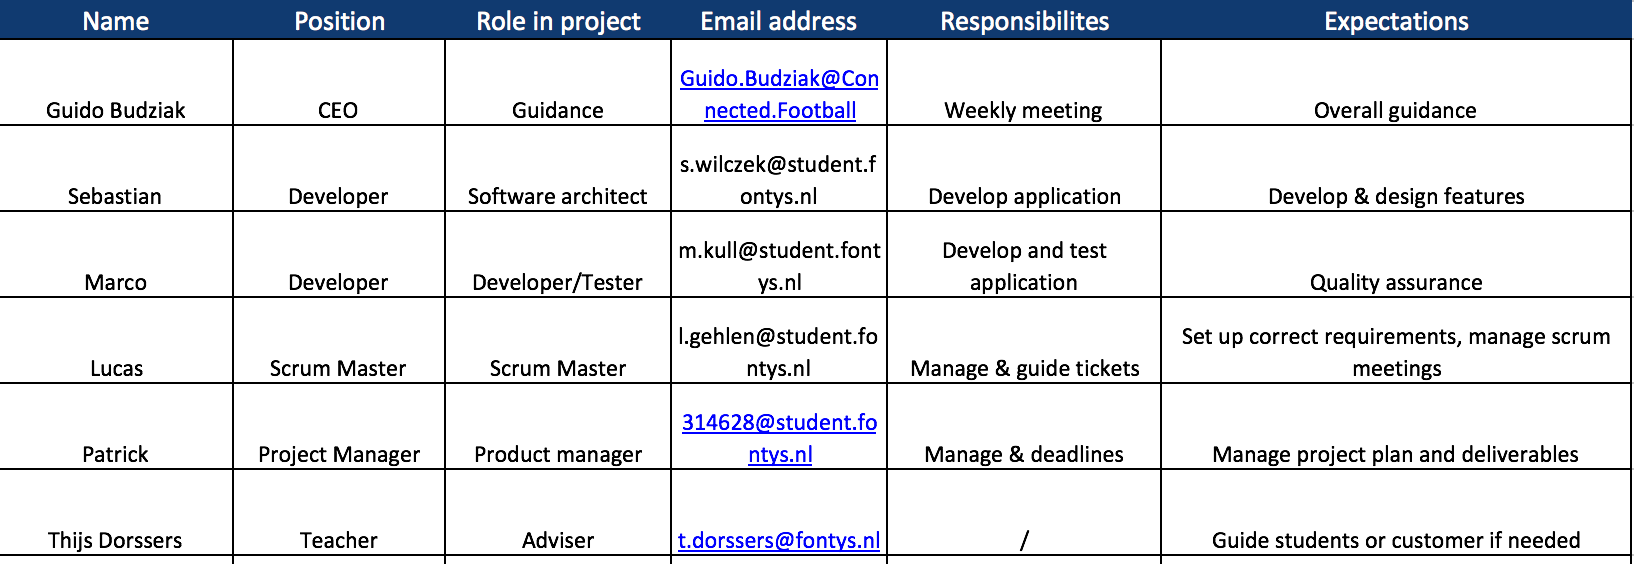
\includegraphics[width=\linewidth]{images/diagrams/human_resc.png}
  \caption{Overview human resource management}
\end{figure}
\newpage

\subsubsection{Develop Project Team}
\label{sssec:develop_project_team}

Developing the Project Team is the process of improving competencies, team member interaction, and overall team
environment to enhance project performance. Over the 14 weeks students have to improve in certain areas. Lucas who is responsible for the scrum management has to study the tech stack with YouTube videos and the official documentation. Marco has to improve his knowledge in the area of web development and testing. Patrick in the role of a project manager should acquire skills to identify, build, maintain, motivate, lead, and inspire project teams
to achieve high team performance and to meet the project’s objectives. 

\subsubsection{Manage Project Team}
\label{sssec:manage_project_team}

Managing the Project Team is the process of tracking team member performance, providing feedback, resolving
issues, and managing team changes to optimize project performance. The project manager tries to identify lacks in knowledge areas and develops a strategy with the student to compensate the lack. Since there is no budget involved, students have to learn from free sources.


%%%%%%%%%%%%%%%%%%%%%%%%%%%%%%%%%%%%%%%%%%%%%%%%%%
%% COMMUNICATION MANAGEMENT
%%%%%%%%%%%%%%%%%%%%%%%%%%%%%%%%%%%%%%%%%%%%%%%%%%

\subsection{Communication Management}
\label{ssec:communication_management}

The overall objective of  Communications Management is to promote the success of a project by meeting the information needs of project stakeholders. The SoFa \textit{Connected.Football} Communications Management defines the project’s structure and methods of information collection, screening, formatting, and distribution and outline understanding among project teams regarding the actions and processes necessary to facilitate the critical links among people, ideas, and information that are necessary for project success.
 
\subsubsection{Stakeholder Identification Analysis}
\label{sssec:stakeholder_identification_analysis}

\begin{table}[H]
    \centering
    \begin{tabular}{|l|l|l|l|l|}
        \hline
        \cellcolor{gray}Name & \cellcolor{gray}Title & \cellcolor{gray}Contact & \cellcolor{gray}Vehicle \\ \hline
        Guido Budziak & Product owner & guido.budziak@connected.football & Slack  \\ \hline
        Marco Kull & Quality Manager & m.kull@student.fontys.nl & Slack    \\ \hline
        Sebastian Wilczek & Software Architect & s.wilczek@student.fontys.nl & Slack   \\ \hline
        Patrick Richter & Project Leader & p.richter@student.fontys.nl & Slack \\ \hline
        Lucas Gehlen & Scrum Master & l.gehlen@student.fontys.nl & Slack   \\ \hline
        Thijs Dorssers & Docent & t.dorssers.fontys.nl & E-Mail   \\ \hline
    \end{tabular}
    \caption{Stakeholder identification}
    \label{tab:stakeholder_identification}
\end{table}

\subsubsection{Communications Vehicles}
\label{sssec:communications_vehicles}

The following table shows the communication matrix of the project. 

\begin{table}[H]
    \centering
    \begin{tabular}{|l|l|l|l|l|l|l}
        \hline
        \cellcolor{gray}Vehicle & \cellcolor{gray}Target & \cellcolor{gray}Purpose & \cellcolor{gray}Frequency & \cellcolor{gray}Owner & \cellcolor{gray}Distribution Vehicle \\ \hline
        Project Plan & All stakeholders & \begin{tabular}{@{}c@{}}The project plan\\for this project\end{tabular} & Once & Project Leader & \textit{SVN} \\ \hline
    \end{tabular}
    \caption{Communication matrix}
    \label{tab:communication_matrix}
\end{table}

\begin{table}[H]
    \centering
    \begin{tabular}{|l|l|l|l|l|}
        \hline
        \cellcolor{gray}Vehicle & \cellcolor{gray}Frequency & \cellcolor{gray}Internal/External & \cellcolor{gray}Initiator  \\ \hline
        Daily & every project day & Internal & Scrum Master     \\ \hline
        Customer meeting & every Tuesday & External & Project Leader  \\ \hline
        Coach meeting & every Tuesday & Internal & Project Team   \\ \hline
        Sprint planing & every Tuesday & Internal & Scrum Master  \\ \hline
        Coach meeting & every Tuesday & Internal & Project Team  \\ \hline
    \end{tabular}
    \caption{Project Meetings}
    \label{tab:project_meetings}
\end{table}

In this project four meetings were identified. First of all there were the daily scrum meeting in which the project team discussed what they have worked on during the most recent project day, what they will do on the current day and if there are any obstacles that stop them from doing their work.
\newline
Then there was the customer meeting in which the project team discussed the progress and obstacles with the customer. The coach meeting informs the coach about the progress and obstacles. Finally in the sprint planning the project team planned the next sprint and decided which issues will be solved in the next sprint. Also, the past sprint was discussed and analysed. 

%%%%%%%%%%%%%%%%%%%%%%%%%%%%%%%%%%%%%%%%%%%%%%%%%%
%% RISK MANAGEMENT
%%%%%%%%%%%%%%%%%%%%%%%%%%%%%%%%%%%%%%%%%%%%%%%%%%

\subsection{Risk Management}
\label{ssec:risk_management}

The following sections deals with the Risk Management. This involved how Risk Management was planned in the context of the project, including how risks were identified for each individual defined Epic.

\subsubsection{Plan Risk Management}
\label{sssec:plan_risk_management}

This chapter describes the project related risks and the impact of these risks to the project. Risk management is a continuous process where risks have to be evaluated continuously with all stakeholders to ensure a proper risk assessment. To execute a proper risk management, there are 5 important steps that needs to be executed.

\begin{enumerate}
    \item Identify the Risk.
    \item Analyse the risk.
    \item Evaluate or Rank the Risk.
    \item Treat the Risk.
    \item Monitor and Review the risk.
\end{enumerate}

Together these 5 risk management process steps combine to deliver a simple and effective risk management process.
In this project only the most relevant risk criteria are assessed even though there are many more risks that could be evaluated.

\subsubsection{Identify Risks}
\label{sssec:identify_risks}

Is the process of determining which risks may affect the project and documenting their characteristics.
As part of the Sofa project the assessment of risks for the three epics in conjunction with our customer.
Continuously analysing and evaluating risks is an important task of project management. Even in early stages of the project evaluated risks can be tackled and occurrence of likelihood minimised.
In this \textit{Connected.Football} project three risk breakdown structures are created.
One for every epic. Three levels of risks are determined, where level one is the epic, level two the involved party and level three the occurring issue. All risks are evaluated against the seriousness and likelihood of occurrence.

\begin{table}[H]
  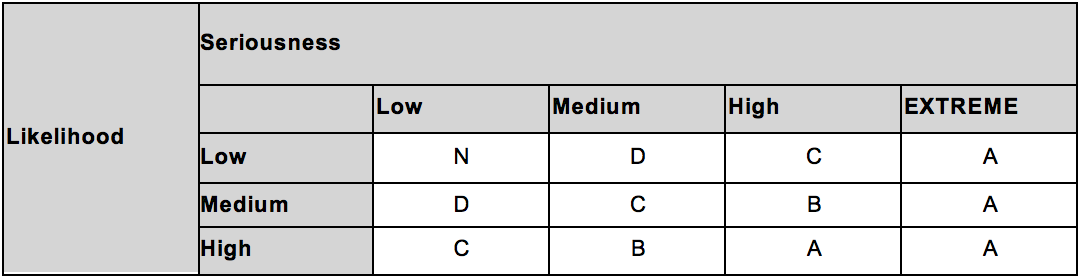
\includegraphics[width=\linewidth]{images/diagrams/risk_grading.png}
  \caption{Risk matrix}
\end{table}

\paragraph{Epic 1}
In the epic "Vote4Fun" the most influential risk is that the group of students is not able to learn the necessary knowledge to integrate the epic of the customer. 
\newline
To ensure that missing knowledge is learned within appropriate time students need to spend time on their own to compensate that knowledge and reduce the likelihood of that risk.

\begin{table}[H]
  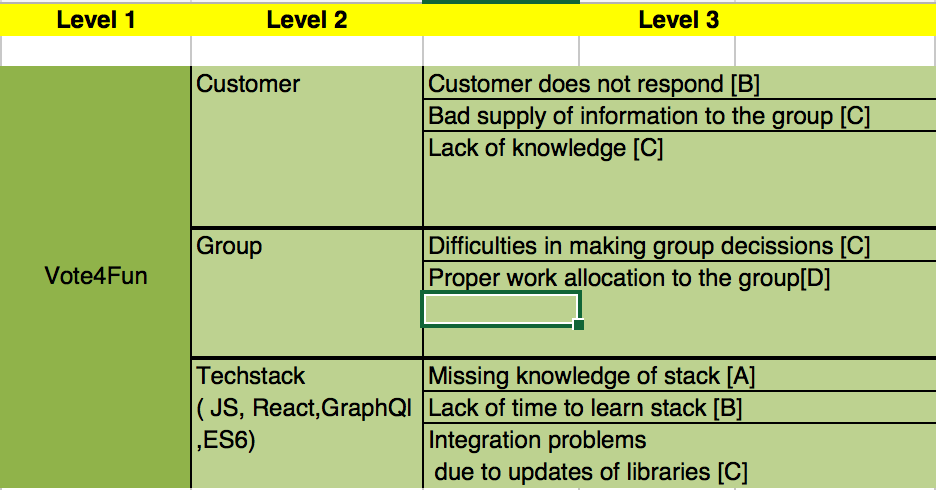
\includegraphics[width=\linewidth]{images/diagrams/vote4fun.png}
  \caption{Epic 1}
\end{table}

\paragraph{Epic 2}
In the epic "Promotion Code" the most influential risk is the lack of knowledge on how to solve and implement the promotion code for certain users to enter the application. 
\newline
To reduce the likelihood of the customer who does not respond students shall deliver quality to the customer to keep him satisfied over the project life cycle.

\begin{table}[H]
  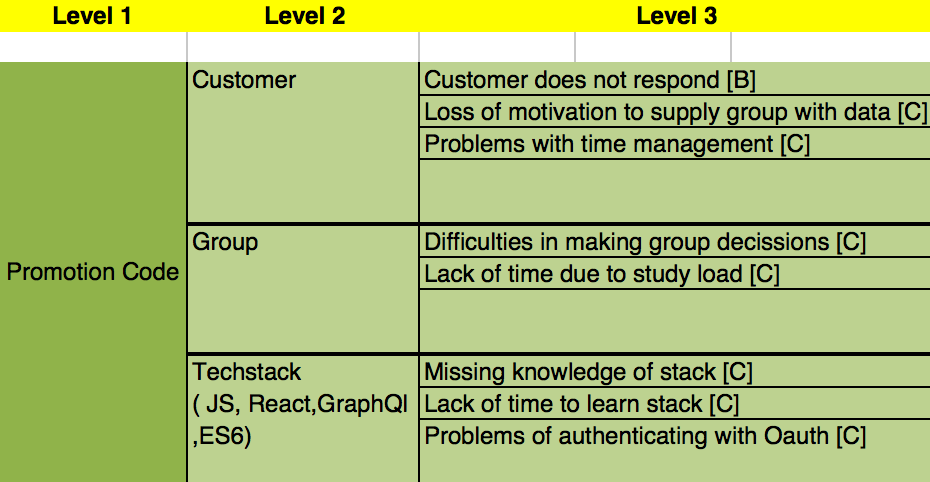
\includegraphics[width=\linewidth]{images/diagrams/promotioncode.png}
  \caption{Epic 2}
\end{table}

\paragraph{Epic 3}
In the Epic "Group extension" the most influential risk is that we run out of time due to the workload of the first two epics. To minimise the likelihood of occurrence that students will encounter problems due to the lack of time students need to have a structured set up of their sprint planning to always have an overview of their current project status.

\begin{table}[H]
  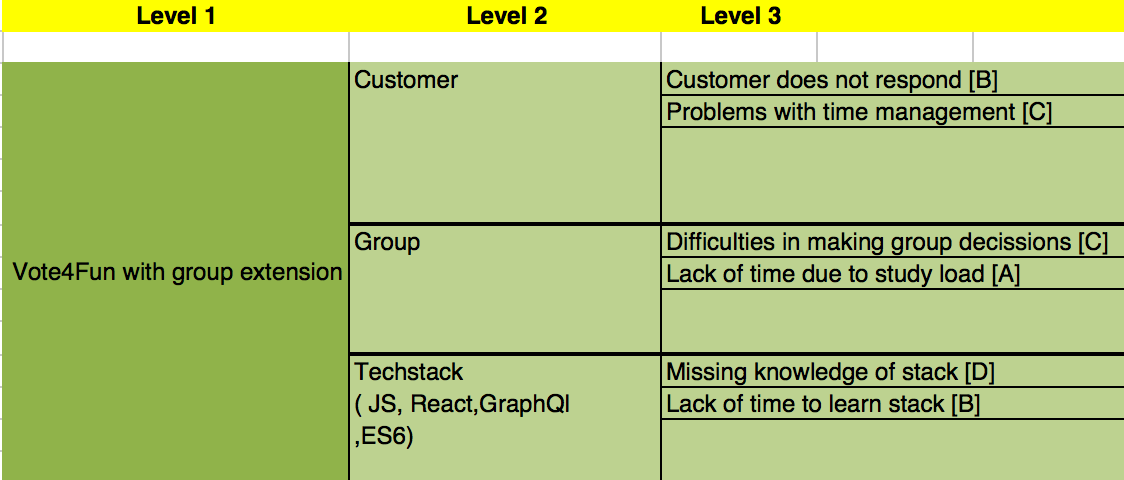
\includegraphics[width=\linewidth]{images/diagrams/groupextension.png}
  \caption{Epic 3}
\end{table}

\subsubsection{Identification}
\label{sssec:identification}

The objective of risk identification is the early and continuous identification of potential risks that can affect the project delivery. It is crucial for efficient risk management. If the risk occurs it would have negative (or sometimes positive) impact on the project's ability to achieve performance or capability outcome goals. Through the whole project life cycle this is an continuously iterative process that needs to be repeated. In the previous chapter the risks got analysed and selected. 


%%%%%%%%%%%%%%%%%%%%%%%%%%%%%%%%%%%%%%%%%%%%%%%%%%
%% PROCUREMENT MANAGEMENT
%%%%%%%%%%%%%%%%%%%%%%%%%%%%%%%%%%%%%%%%%%%%%%%%%%

\subsection{Procurement Management}
\label{ssec:procurement_management}

Part of the Project Management process is to manage the processes necessary to acquire services and products that ensure the ability to work on the project. This includes both management services as well as external software products used in development.
\newline
The project encompassed the following products and services. It is detailed how they were used in the project and who was responsible for providing them.

\subsubsection{Atlassian \textit{Jira}}
\label{sssec:jira}

\begin{figure}[H]
    \begin{center}
        
\includegraphics[width=0.3\textwidth]{images/logos/jira-logo.png}
        \caption{Atlassian \textit{Jira} Logo}
        \label{fig:jira_logo}
    \end{center}
\end{figure}

To manage the agile process of the project, \textit{Jira} by Atlassian was made use of. The platform allowed the project team members to keep track of the backlog of tasks and user stories and to manage them in Scrum sprints.
\newline
\textit{Jira} was provided by the client \textit{Connected.Football}. The client was responsible for granting the other team members and stakeholders access to the tool and to ensure that certain team members have the necessary permissions to interact with the provided tool set. The developing team members were responsible for keeping the content of the created \textit{Jira} boards correct and up-to-date.

\subsubsection{\textit{GitHub}}
\label{sssec:github}

\begin{figure}[H]
    \begin{center}
        
\includegraphics[width=0.2\textwidth]{images/logos/github-logo.png}
        \caption{\textit{GitHub} Logo}
        \label{fig:github_logo}
    \end{center}
\end{figure}

The developed \textit{React Native} product was being versioned using \textit{Git}, which uses \textit{GitHub} as a platform. The client was again responsible for providing the team members access to the versioning system and to ensure that the provided sources are in a state that enables development by the project team.
\newline
The project team was responsible for committing changes they make to the product to the \textit{GitHub} repository, including accurate descriptions of what has been changed since the last commit. It was also the responsibility of the team to resolve commit errors and conflicts, as well as to minimise the likelihood of such occurrences.

\subsubsection{\textit{Subversion}}
\label{sssec:subversion}

Another versioning system used over the course of the project was \textit{Subversion}. This system was used to commit and share University-related artefacts and documents, such as this project report.
\newline
Fontys Hogeschool Techniek en Logistiek Venlo was responsible for the availability and integrity of the repositories in question. Again, it was the responsibility of the team members to ensure a working state of the repositories and to commit changes with accurate descriptions.

\subsubsection{\textit{Firebase}}
\label{sssec:firebase}

\begin{figure}[H]
    \begin{center}
        
\includegraphics[width=0.2\textwidth]{images/logos/firebase-logo.png}
        \caption{\textit{Firebase} Logo}
        \label{fig:firebase_logo}
    \end{center}
\end{figure}

Some backend functionality of the product was relying on Google's \textit{Firebase}. It was for example used to send push notifications to mobile user devices.
\newline
It was the responsibility of the client to ensure that the project team has the necessary rights to interact with the already set up \textit{Firebase} backend. On the other hand, the team was responsible for interacting with the backend in a proper way, ensuring the integrity of the provided data and infrastructure. The project team did not have any access to the backend in the sense of interacting with the interface provided by Google, but by using it by referencing and using it in the source code of the application.

\subsubsection{Integrated development environments}
\label{sssec:ides}

\begin{figure}[H]
    \begin{center}
        
\includegraphics[width=0.2\textwidth]{images/logos/visual-studio-code-logo.png}
        \caption{\textit{Visual Studio Code} Logo}
        \label{fig:visual-studio-code_logo}
    \end{center}
\end{figure}

The project team used some integrated development environments (IDEs) to develop the product, most notably \textit{Visual Studio Code}. The IDE was used to inspect and change the source code of the product.
\newline
The developer was responsible for the functionality of the IDE. The team was able to use the IDEs as they are all provided through open source. It was their responsibility to use the IDE as intended and to figure out how to resolve errors in the event that they occur. No such errors occurred during the course of the project.

\subsubsection{\textit{Node.js} Modules}
\label{sssec:nodejs_modules}

\begin{figure}[H]
    \begin{center}
        
\includegraphics[width=0.3\textwidth]{images/logos/node-js-logo.png}
        \caption{\textit{Node.js} Logo}
        \label{fig:node-js-logo}
    \end{center}
\end{figure}

The product used various \textit{Node.js} modules to offer functionality in the product. These modules were available from various repositories.
\newline
The developers of the \textit{Node.js} modules were responsible for the development of the \textit{Node.js} modules themselves and for the documentation that comes with them. Since the modules were published as open source, the project team is responsible for handling errors that occurred during the development involving their usage. They were furthermore responsible for implementing the usage of the modules in the product as the developer intended and documented.
\newline
Some of the \textit{Node.js} modules were developed by the client. Their integrity was therefore their responsibility.

\subsubsection{\textit{Slack}}
\label{sssec:slack}

\begin{figure}[H]
    \begin{center}
        
\includegraphics[width=0.2\textwidth]{images/logos/slack-logo.png}
        \caption{\textit{Slack} Logo}
        \label{fig:slack-logo}
    \end{center}
\end{figure}

The development team used \textit{Slack} to communicate outside of personal meetings, both in communication with each other as well as with the client. It was also used to share information, such as documents and source code snippets, in a non-persistent way. Configuration files that were not supposed to be uploaded to \textit{GitHub} were also shared using \textit{Slack}.
\newline
The availability of the application was ensured by the developer. It was the responsibility of the client to enable that the development team is able to join and use the \textit{Slack} platform. The project team had the responsibility to not share any sensitive information, such as credentials, over this platform.